\documentclass[12pt]{article}

%Russian-specific packages
%--------------------------------------
\usepackage[T2A]{fontenc}
\usepackage[utf8]{inputenc}
\usepackage[english, russian]{babel}
%for search in russian
\usepackage{cmap}
% for quotes
\usepackage{csquotes}
%--------------------------------------

%Math-specific packages
%--------------------------------------
\usepackage{amsmath}
\usepackage{amssymb}

\def\d{ \mathrm{d} }

\usepackage{amsthm}
\newtheorem{lemma}{Лемма}
\newtheorem{definition}{Определение}
\newtheorem*{remark}{Замечание}

%Format-specific packages
%--------------------------------------
\usepackage[left=2cm,
            right=2cm,
            top=1cm,
            bottom=2cm,
            bindingoffset=0cm]{geometry}

%Graphics packages
%--------------------------------------
\usepackage{graphicx}
\usepackage{wrapfig}

\graphicspath{ { ./tex/ } }

\includeonly{
  tex/title
  , tex/introduction
}

\usepackage{tikz}
\usetikzlibrary{
  shapes.geometric
  , intersections
  % for angles
  , angles
  , quotes
  , babel
  % ------
}

\begin{document}

\begin{titlepage}
  \begin{center}
    \large{Федеральное государственное бюджетное образовательное\\
      учреждение высшего образования\\}

    Московский государственный университет\\
    имени М. В. Ломоносова\\

    \vspace{0.25 cm}

    \normalsize{Механико-математический факультет\\}
    \vspace{0.5 cm}
    Кафедра вычислительной математики\\
  \end{center}

  \vspace{3cm}

  \begin{center}
    \LARGE{Курсовая работа}\\

    \vspace{0.5 cm}

    \normalsize{}
    \textbf{Тема:} \textit{Введение в Photometric Stereo.}
  \end{center}

  \vspace{3 cm}

  \begin{flushright}
    \textbf{Выполнил:}\\
    студент 4 курса
    431 группы\\

    \textit{Шерстобитов Андрей Сергеевич}\\

    \vspace{1 cm}

    \textbf{Научный руководитель:}\\

    \textit{Валединский Владимир Дмитриевич}
  \end{flushright}

  \vspace{\fill}
  \normalsize{}
  \begin{center}
    Москва\\2022
  \end{center}

  \thispagestyle{empty}
\end{titlepage}


\newpage
\tableofcontents

\newpage

\section{Вступление}

Photometric stereo — метод в компьютерном зрении для определения
нормалей поверхности объектов путем наблюдения за этим объектом
при различных условиях освещения. Он основан на том факте,
что количество света, отражаемого поверхностью, зависит от ориентации
поверхности относительно источника света и наблюдателя.

\begin{figure}[h]
  \centering
  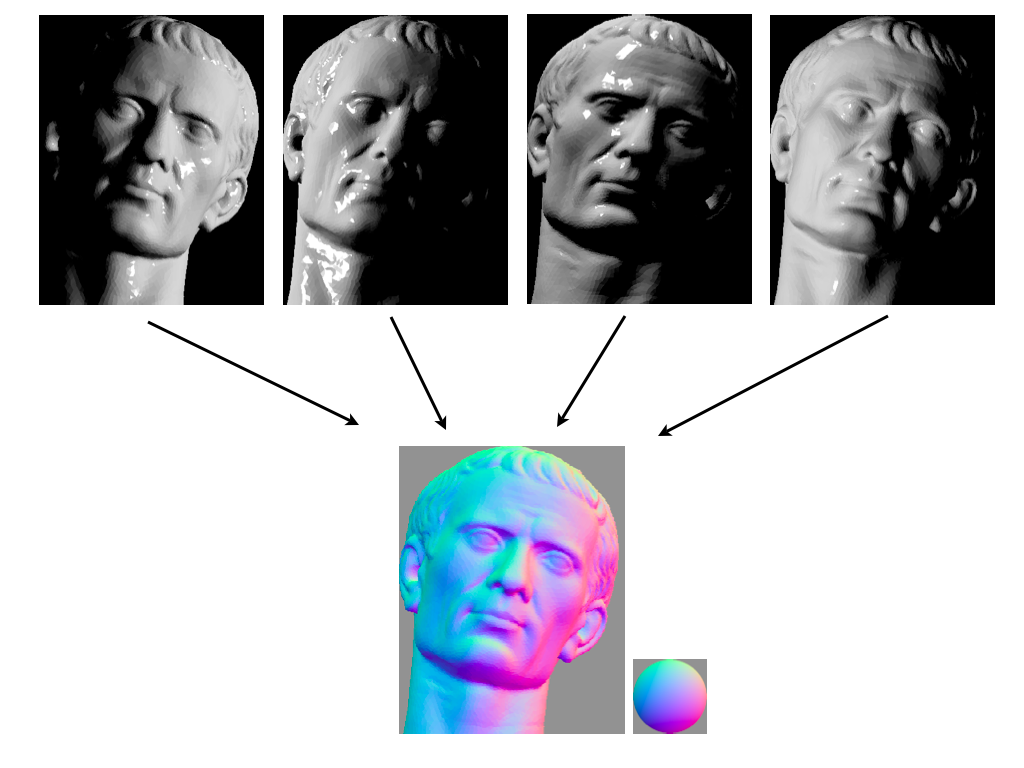
\includegraphics[scale=0.3]{tex/example.png}
\end{figure}

При использовании этого метода путем измерения количества света,
отраженного в камеру, пространство возможных ориентаций поверхности может
быть ограничено. Если объект наблюдается под достаточным количеством источников
света с разных углов, то ориентация поверхности может быть ограничена
до одной ориентации или даже получиться больше, чем необходимо.

Метод был впервые предложен в 1980 году Уодхэмом. Особый случай,
когда данные представлены одним изображением, известен как "shape from shading",
и был анализирован Б. К. П. Хорном в 1989 году. Расширенные методы фотометрического
стерео были разработаны для учета проецируемых теней и других
неоднородных условий освещения.

Однако, этот метод требует тщательного планирования и контроля эксперимента,
чтобы получить необходимое количество данных, и считается,
что он неэффективен для объектов с неоднородной поверхностью
и большим числом полостей. Тем не менее, photometric stereo все еще остается
важной технологией в области компьютерного зрения, особенно для задач
реконструкции трехмерных объектов.


\newpage

\section{Радиометрия}
\subsection{Телесный угол}

Познакомимся с понятием \textit{телесного угла}, разберемся как и в чем происходит измерение этой величины. Именно с него будет начинаться наше погружение
в Photometric stereo.

\begin{wrapfigure}[14]{r}{0.4\textwidth}
  \begin{center}
    \begin{tikzpicture}[scale=0.9,every node/.style={scale=0.9}]
      \draw (0,0) circle (2cm);
      \coordinate [label=below:$O$] (O) at (0,0);
      \draw [dashed] (0,0) -- node[above]{$R$} (-2,0);
      \draw (-2,0) arc (180:360:2 and 0.6);
      \draw [dashed] (2,0) arc (0:180:2 and 0.6);

      \node [ellipse,
        draw=black,
        fill=cyan!10,
        minimum width = 0.6cm,
        minimum height = 0.4cm,
        rotate=125] (e) at (0.9,0.9) {};
      \draw [dashed] (O) -- (e.east);
      \draw [dashed] (O) -- (e.west);

      \node [ellipse,
        draw=black,
        fill=cyan!20,
        minimum width = 1.8cm,
        minimum height = 1.2cm,
        rotate=125] (E) at (2.70,2.70) {};
      \draw (e.east) -- (E.east);
      \draw (e.west) -- (E.west);
      \coordinate [label=center:$\Sigma$] (S) at (E.center);

    \end{tikzpicture}
    \caption{Телесный угол}
  \end{center}
\end{wrapfigure}

Поставим наблюдателя в центр сферы $O$ радиуса $R$. Обозначим $\Sigma$ наблюдаемую
из точки $O$ поверхность. Площадь сферы покрываемую объектом обозначим $S$. Тогда величиной телесного угла
является следующее отношение:
$$\omega=\frac{S}{R^2}$$
Точка $O$ называется вершиной (apex) телесного угла.
\textbf{Телесный угол} - пучок лучей из $O$ до $\Sigma$.
Говорят, что наблюдатель стягивает (to subtend) его телесный угол в вершине.

Единица измерения в системе  СИ - стерадиан (sr), равный телесному углу,
вырезающему из сферы радиуса $R$ поверхность с площадью $R^2$.

\begin{remark}
  Площадь поверхности сферы = $4\pi R^2$, тогда полный телесный угол равен
  $$\omega=\frac{4\pi R^2}{R^2}=4\pi$$
\end{remark}

\begin{remark}
  Для кругового конуса с углом раствора $\theta$ телесный угол при его вершине
  равен $$\omega=\frac{2\pi R^2(1-\cos\theta)}{R^2}=2\pi(1-\cos\theta)$$
\end{remark}

\begin{wrapfigure}[10]{r}{0.35\textwidth}
  \begin{center}
    \begin{tikzpicture}[scale=0.75]
      \coordinate (O) at (0,0);
      \node [circle,
        name path=U,
        draw=black,
        minimum size=3cm] (U) at (O) {};
      \node [circle,
        draw=black,
        label=left:$S_0$] (S0) at (O) {};

      \coordinate (dAl) at (1,-7);
      \coordinate (dAr) at (3,-7);
      \coordinate (dAm) at (2,-7);
      \coordinate (n) at (2,-6);
      \draw (dAl) -- (dAr);

      \draw [name path=O--dAl,dashed] (O) -- node [left] {$r$} (dAl);
      \draw [name path=O--dAr,dashed] (O) -- (dAr);
      \draw (O) -- (dAm) node [below] {$\d A$};

      \begin{scope}
        \path [name intersections={of=O--dAl and U,by=C}];
        \path [name intersections={of=O--dAr and U,by=D}];
        \draw [line width=1mm] (C) -- (D) node [right] {$\d A_0$};
      \end{scope}

      \draw [->, line width=0.5mm] (dAm) -- (n) node [right] {$\mathrm{n}$};
      \pic [draw, angle radius=6mm,"$\theta$",left] {angle=n--dAm--O};
    \end{tikzpicture}
    \caption{Стянутый объектом $S_0$ телесный угол}
    \label{subtended}
  \end{center}
\end{wrapfigure}

Чаще всего бывает, что изучаемая поверхность находится под углом $\theta$
к наблюдателю. На рис. \eqref{subtended} $\mathrm{n}$ это нормаль к
изучаемой поверхности $\d A$, $S_0$ - центр единичной окружности.
Расстояние между $S_0$ и $\d A$ обозначим $r$. Заметим, что угол между
нормалью плоскости $\mathrm{n}$ и направлением взгляда наблюдателя обозначим $\theta$.
$\d A_0$ является проекцией $\d A$ на единичную сферу, тогда телесный угол имеет величину:
$$\d \omega = \frac{\d A\cos\theta}{r^2}$$

\newpage

\subsection{Сила света (Intensity)}

Простыми словами фотометрия - наука об измерении света с точки
зрения его яркости, воспринимаемой человеческим глазом.
Сразу можно задать вопрос: как и в чем измеряется
свет? Попытаемся формализировать ответы на эти вопросы.

%До 1948г. существовали различные стандарты измерения силы света, в основном зависящие
%от выбранного источника света. Только
% В 1948г. физик Жюль Виоль предложил способ измерения силы света, которое
% используется и по сей день

Современное определение единицы силы света было зафиксировано в 1979 г.
XVI Генеральной конференцией по мерам и весам. Международной системе единиц (СИ)
имеет следующее описание:

\begin{displayquote}
  Сила света в заданном направлении источника, испускающего
  монохроматическое излучение частотой 540$\cdot$1012 Гц, энергетическая сила света
  которого в этом направлении составляет 1/683 Вт/ср.
\end{displayquote}

Единица силы света имеет общеприниятое название -- кандела (кд, cd).
Сила света имеет обозначение $I$.

Для силы света оказался верен закон обратных квадратов: значение силы света в
данной точке пространства обратно пропорицонально квадрату расстояния от источника света.
То есть имея два источника света с соотвествующими силами $I_1$ и $I_2$, расположенные
соответственно на расстояних $r_1$ и $r_2$ верно следующее равенство:

\begin{equation}
  \frac{I_1}{I_2} = \frac{r_2^2}{r_1^2}
\end{equation}

\subsection{Поток (Flux)}

Рассмотрим некоторый источник света $S_0$ в некотором пространстве.
Излучаемый свет можно представить как совокупность телесных углов $\omega$ с вершиной
в источнике $S_0$.


\subsection{Облученность (Irradiance)}

\subsection{Энергетическая яркость (Radiance)}

По определению яркость излучения это отношение

\newpage

\section{Литература}
\begin{enumerate}
  \item Гуревич М. М. Фотометрия. Теория, методы и приборы. — 2-е изд. — Л.: Энергоатомиздат. Ленинградское отделение, 1983. — С. 23—24. — 272 с.
  \item Ying Wu. "Radiometry, BRDF and Photometric Stereo". Northwestern University. Retrieved 2015-03-25.
  \item A. V. Arecchi, T. Messadi, and R. J. Koshel, Field Guide to Illumination, SPIE Press, Bellingham, WA (2007)
\end{enumerate}
\end{document}
